\documentclass[a4paper,11pt]{report}
\usepackage[T1]{fontenc}
\usepackage[utf8]{inputenc}
\usepackage[polish]{babel}
\usepackage{lmodern}
\usepackage{graphicx}

\title{czas obsługi: tablicy asocjacyjnej}
\author{Tomasz Piotrowski 200524}

\begin{document}
\maketitle
\begin{figure}
\textbf {\Large{ Sprawozdanie z czasu obsługi talbicy asocjacyjnej wykonanej na trzech strukturach:\\
-vektor\\
-drzewo wyszukiwan binarnych\\
-tablica haszujaca\\
. }}
\end{figure}


\begin{figure}
Zmierzony został czas dostepu do elementu w tablicy asocjacyjnej zaimplementowanej na roznych stukturach. Ponieważ czas dostępu do elementu jest bardzo mały funkcja szukajaca elementu wywolana zostala mln razy. Wyniki pomiarow zaprezentowane zostały na wykresie, oraz w tableli
\end{figure}


\begin{figure}

  \begin{center}
	
  
  
    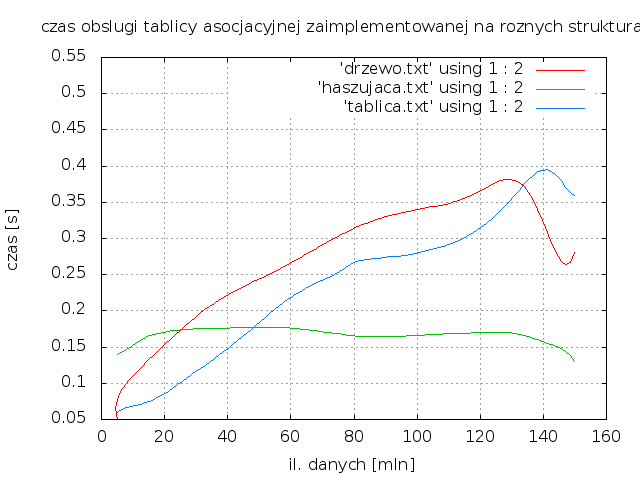
\includegraphics[scale=0.5]{./czas_dzialania_algorytmow.png}
    \label{fig:}
    \caption{}
 
          \begin{tabular}{|l|c|c|r|}
\hline
il[mln] & czas drzewo [s] & haszujaca& vector \\
5.000000 & 0.05& 0.14&0.06\\
1.0000000 &  0.11& 0.14& 0.08\\
15.000000  & 0.11& 0.2&0.06\\
20.000000  & 0.16& 0.16&0.08\\
25.000000  & 0.17& 0.17&0.06\\
30.000000  & 0.22& 0.18& 0.21\\
35.000000 &  0.18& 0.2&0.09\\
40.000000  & 0.24& 0.14&0.09\\
45.000000  & 0.31& 0.19&0.21\\
50.000000  & 0.17& 0.19& 0.21\\
55.000000  & 0.22& 0.15&0.08\\
60.000000  & 0.34& 0.2&0.31\\
65.000000  & 0.22& 0.2& 0.42\\
70.000000  & 0.29& 0.15&0.08\\
75.000000  & 0.35& 0.19&0.11\\
80.000000  & 0.29& 0.14& 0.51\\
85.000000  & 0.35& 0.14&0.22\\
90.000000  & 0.35&  0.17&0.08\\
95.000000  & 0.3& 0.17& 0.38\\
100.000000 &  0.36& 0.18&0.43\\
105.000000 &  0.35& 0.15&0.18\\
110.000000 &  0.36& 0.19&0.1\\
115.000000 &  0.36 & 0.15&0.48\\
120.000000 &  0.24& 0.17&0.11\\
125.000000 &  0.42&  0.17&0.5\\
130.000000 &  0.46&  0.19&0.18\\
135.000000 &  0.48& 0.18&0.47\\
140.000000 & 0.28&  0.13&0.46\\
145.000000 &  0.22& 0.17&0.36\\
150.000000 &  0.28&  0.13&0.36\\
\hline


\hline
\end{tabular}
\newline

  \end{center}
\end{figure}
\begin{figure}
Na podstawie wykresu można stwierdzić że tablica asocjacyjna zaimplementowana na tablicy haszujacej jest najkorzystniejsza ponieważ czas dostępu do elementu w przybliżeniu jest liniowy. 
W przypadku talbiy asocjacyjnej zaimplementowanej na drzewie binarnym oraz na vektorze sortowanym i przeszukiwanym binarnie czas dostepu do szukanego elementu jest podobny. 
Z tabeli można wywnioskować że w przypadku vectora oraz drzewa binarnego czas wyszukiwania zależny jest nie tylko od ilości elementów oraz również od wartości klucza to znaczy od położenie poszukiwanego elementu w całej tablicy. 
\end{figure}

\end{document}
